\documentclass[article,12pt,onesidea,4paper,english,brazil]{abntex2}

\usepackage{lmodern, indentfirst, nomencl, color, graphicx, microtype, lipsum}			
\usepackage[T1]{fontenc}		
\usepackage[utf8]{inputenc}		
\usepackage{commath}
\setlrmarginsandblock{2cm}{2cm}{*}
\setulmarginsandblock{2cm}{2cm}{*}
\checkandfixthelayout

\setlength{\parindent}{1.3cm}
\setlength{\parskip}{0.2cm}

\SingleSpacing

\begin{document}
	
	\selectlanguage{brazil}
	
	\frenchspacing 
	
	\begin{center}
		\LARGE TÍTULO DO RESUMO
		
		\normalsize
	Luís HenriqueAmaroVéras\footnote{Discente do curso técnico integrado em eletrotécnica, e-mail: lauramlk2@gmail.com, Campus Calama .} 
	Laura Raisa de Carvalho\footnote{Discente do curso técnico integrado em eletrotécnica, e-mail: amaroveras@outlook.com, Campus Calama } 
	Eloisa Silva de Jesus\footnote{Discente do curso técnico integrado em química, e-mail: emilyingridb@gmail.com, Campus Calama } 
		Emily Ingrid Bader de Souza Rômer\footnote{Discente do curso técnico integrado em química. E-mail: Lais\_k5@hotmail.com, Campus Calama } 
	Natália Thais Bukoski Silva\footnote{Discente do curso técnico integrado em química, E-mail: naty.thais65@gmail.com,Campus Calama } 
	Lais Souza Pinto
	
	\footnote{Orientador,raimundo.santos@ifro.edu.br, Campus Calama} 
	\end{center}
	
	% resumo em português
	\begin{resumoumacoluna}
		: O presente trabalho foi feito para pesquisar a quantidade de estudantes  de escolas da cidade de Porto Velho que usam ou consomem algum tipo de droga. Podemos notar uma grande quantidade de usuários de drogas licitas.
		
		
		
		\vspace{\onelineskip}
		
		\noindent
		\textbf{Palavras-chave}: drogas, estudantes, Porto Velho.
	\end{resumoumacoluna}
	
	\section*{Introdução}
	
Em um novo século, novas tecnologias surgem, novos computadores, novos estilos, novas comidas, novas bebidas e até mesmo, novas drogas. O mundo evolui e junto com ele, boas e más ciências também, sendo comum que haja interesse e uma enorme vontade de conhecer esse novo plano e suas virtudes. Com toda essa inovação, as pessoa vão atrás de algo que as faça sentir-se bem, buscando principalmente bebidas e álcool, pois com o seu consumo elas podem ter uma ilusória visão de que tudo está bem ou fingir que nada aconteceu. Simplesmente, esquecer e viver o momento de diversão, como muitas costumam relatar.

Essas experiências fazem com que a procura de drogas, sendo elas lícitas ou ilícitas seja frequente, independente da idade, causando muitas vezes dependências e vícios, os quais são na maioria das vezes decorrentes de problemas familiares, amigos, depressão, transtornos, entre outros. Sendo de alta importância para a saúde pública, palestras e incentivos contra o uso dessa drogas, pois um alto uso pode resultar em doenças e até mesmo a morte.

Quando se fala sobre os temas "Drogas e Álcool", o assunto vai muito além do que simples números, trata-se de saúde, violência e também suicídio, e é visando esses pontos que torna-se de extrema importância, a coleta de dados reais sobre usuários de álcool e drogas nas escolas de ensino médio, sendo elas públicas, federais ou particulares,pois é na adolescência onde ocorre um maior índice de curiosidade e atração para conhecer o novo, podendo ser até mesmo por influencia dos amigos.


	
	\section*{Material e Método}
	
O material usado foi parcialmente tirado dos próprios alunos e artigos já publicados sobre isso

A pesquisa foi desenvolvida nas escolas de ensino médio do município de Porto Velho, e teve como meta demonstrar o índice de uso de drogas entre os jovens, apontando a dimensão do problema para que se possa sugerir às autoridades municipais a promoção de medidas de combate e conscientização do mesmo. O tratamento estatístico dos dados levantados aponta o perfil comportamental dos alunos nas escolas pesquisadas, no que diz respeito ao uso de drogas, permitindo uma amostragem da conduta dos jovens estudantes do município de Porto Velho.

A pesquisa foi realizada com 300 alunos (as) do Ensino Médio da rede Federal, Estadual e Privada do Município de Porto Velho, por meio de questionário contendo 24 questões. Dos 300 alunos (as) participantes da pesquisa 100 alunos (as) pertenciam a Rede Estadual; 100 alunos (as) Rede Federal e 100 alunos (as) Rede Privada.
	
	\section*{Resultados e Discussão}
	
A pesquisa realizada revela que do total de alunos avaliados, 114 são do sexo masculino e 147 do sexo feminino; 39 não indicaram o sexo. Do total, 181 alunos afirmaram já ter usado algum tipo de droga, inclusive lícitas, como álcool e cigarro, e 119 afirmou nunca ter usado droga alguma.
\begin{figure}[h]
	\centering
	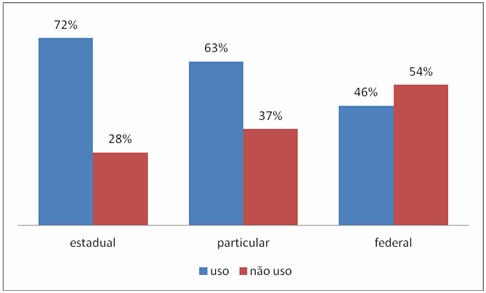
\includegraphics[width=0.7\linewidth]{pip-artigo13-01}
	\caption{índice de usuários}
	\label{fig:pip-artigo13-01}
\end{figure}

Um dado que se revelou surpreendente foi a quantidade de alunos do sexo feminino que são usuários de drogas lícitas e ilícitas. Conforme o gráfico nº 2, nas escolas estaduais 71\% dos usuários são do sexo feminino e 24\% são do sexo masculino; 5\% não indicou o sexo. Na instituição federal, 44\% dos usuários são do sexo feminino e 26\% são do sexo masculino; 26\% não indicou o sexo. Nas instituições privadas o número de usuários é maiormente masculino, sendo 60\% o índice de rapazes usuários de drogas e 32\% de moças; 8\% não indicaram o sexo.
\begin{figure}[h]
	\centering
	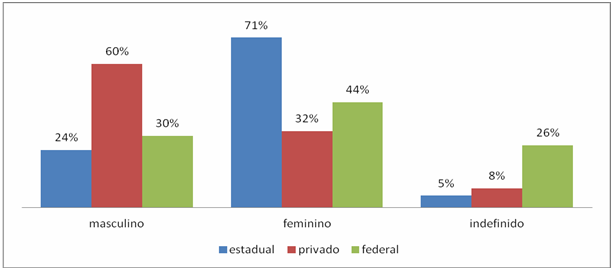
\includegraphics[width=0.7\linewidth]{pip-artigo13-02}
	\caption{Gênero}
	\label{fig:pip-artigo13-02}
\end{figure}

	Também fica demonstrado pela pesquisa que o maior índice de uso de drogas situa-se na rede estadual de ensino. Como a maior parte do alunado é do sexo feminino, gênero no qual se encontra maior índice de usuários de drogas.
	
	Nossos objetivos eram poder ter uma noção de como é a vida dos alunos fora da escola, conseguimos perceber que muda sim de uma escola para a outra, e a maior mudança ou a que mais chamou atenção foi de que eles tem sua origem de uso muito diferente, portanto podemos ver que o tipo de escola muda também o tipo de consumidor, e o que ele(a) consome.
	\section*{Conclusões}
	
A comunidade vem evoluindo muito desde o seu reconhecimento como sociedade, seja criando produtos ou descobrindo novos medicamentos. Mas, ainda com todo conhecimento e explicação que as autoridades dão para a mesma, ainda existem muitos assuntos que precisam ser revisados e ter uma solução. O problema das drogas de uso licito ou ilícito é um dos assuntos que ainda requerem um olhar especial do governo, pois são sim usadas de forma indiscriminada e vão prejudicar quem utiliza e quem convive com o usuário.
	

	\section*{Referências}
	
	\noindent CAVALCANTE, M. B. de P. T; ALVES, M. D. S; BARROSO, M. G. T. ADOLESCÊNCIA, ÁLCOOL E DROGAS: UMA REVISÃO NA PERSPECTIVA DA
	PROMOÇÃO DA SAÚDE. Esc Anna Nery Rev Enferm 2008 set; 12 (3): 555-59
	
	\noindent REIS, F.C; SILVA, A. A - ADOLESCÊNCIA: CONSUMO DE ÁLCOOL E
	OUTRAS DROGAS. Revista enfermagem integrada
	
	\noindent MINAY, M. C. de S; DESLANDES, S. F. A COMPLEXIDADE DAS RELAÇÕES
	ENTRE DROGAS. ÁLCOOL E VIOLENCIACad. Saúde Públ., Rio de Janeiro, 14(1):35-42, jan- mar, 1998
	
	.
	
\end{document}